\documentclass[11pt,a4paper]{article}
\usepackage[utf8]{inputenc}
\usepackage{amsmath,amssymb,graphicx,booktabs,hyperref,siunitx,geometry,float}
\geometry{margin=1in}
\hypersetup{colorlinks=true,linkcolor=blue,urlcolor=blue}

\title{Tutorial 6: Free Surface Flow (Bubble Rise)}
\author{Sajeev \\ CLL769: Applications of CFD}
\date{August 2025}

\begin{document}
\maketitle

\section{Problem Statement \& Objective}
The objective is to perform 2D numerical simulations of a single air bubble rising in a quiescent liquid (water) using the Volume of Fluid (VOF) method. The system involves a rectangular domain ($30$ mm width $\times 72$ mm height). An initial $6$ mm diameter air bubble is located $0.5$ diameters above the bottom wall. 
Phases: 
\begin{itemize}
    \item Primary: Water ($\rho=998.2$ kg/m$^3$, $\mu=0.0012$ kg/m-s).
    \item Secondary: Air ($\rho=1.225$ kg/m$^3$, $\mu=1.789\times 10^{-5}$ kg/m-s).
    \item Surface tension $\sigma = 0.072$ N/m.
\end{itemize}

\section{Computational Setup}
A pressure outlet ($0$ Pa gauge) is applied to the top edge, while the side and bottom edges are modeled as walls (no-slip). The Volume of Fluid (VOF) multiphase model with explicit formulation is used, alongside the Laminar viscous model.
A pressure-based, transient, planar solver is utilized with the PISO algorithm for pressure-velocity coupling. Spatial discretization employs PRESTO! (Pressure) and QUICK (Momentum). Interface reconstruction is handled via Geometric Reconstruction, and a 1st Order Implicit transient formulation ($\Delta t = 10^{-5}$ s) is applied.

\section{Geometry, Meshing \& Initial State}
A uniform grid was used to ensure 8 cells per bubble diameter ($6\text{ mm}/8 = 0.75\text{ mm}$). The air bubble was initialized by patching a circular region with a volume fraction of 1.
\begin{figure}[H]
    \centering
    
\includegraphics[width=0.4\linewidth]{../mesh.png}
    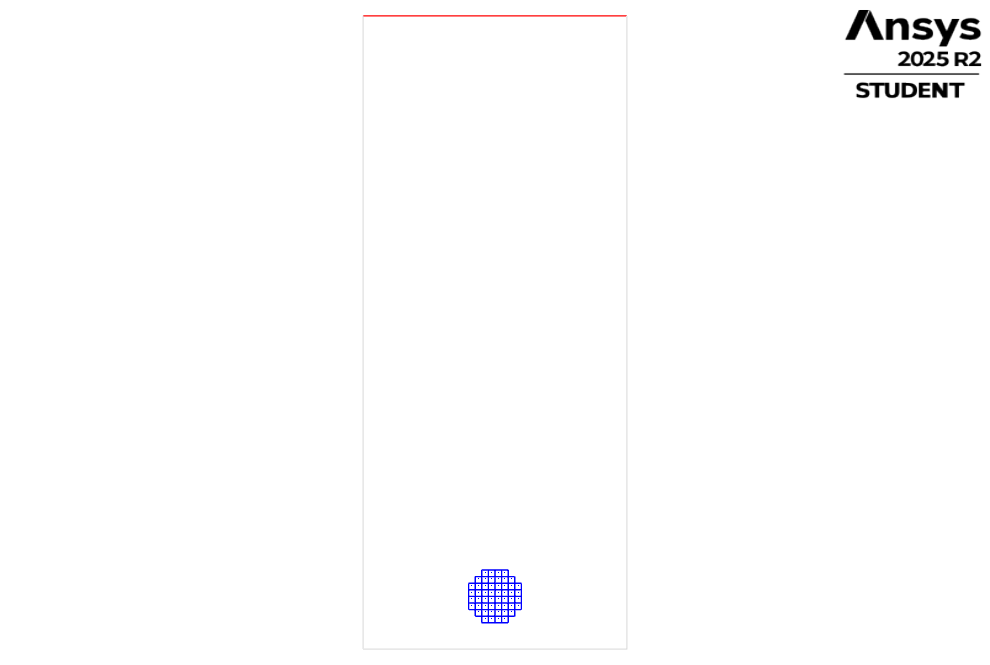
\includegraphics[width=0.4\linewidth]{../bubble_patch.png}
    \caption{Uniform grid (left) and initial bubble patch at $t=0$ (right).}
\end{figure}

\section{Results \& Discussion}
\subsection{Transient Rise Dynamics}
The VOF method and Geometric Reconstruction scheme successfully capture the interface deformation over time. The bubble transitions from its initial spherical shape into a dimpled/skirted shape due to hydrodynamic forces dominating over surface tension, consistent with the Clift et al. bubble shape regimes. 

\begin{figure}[H]
    \centering
    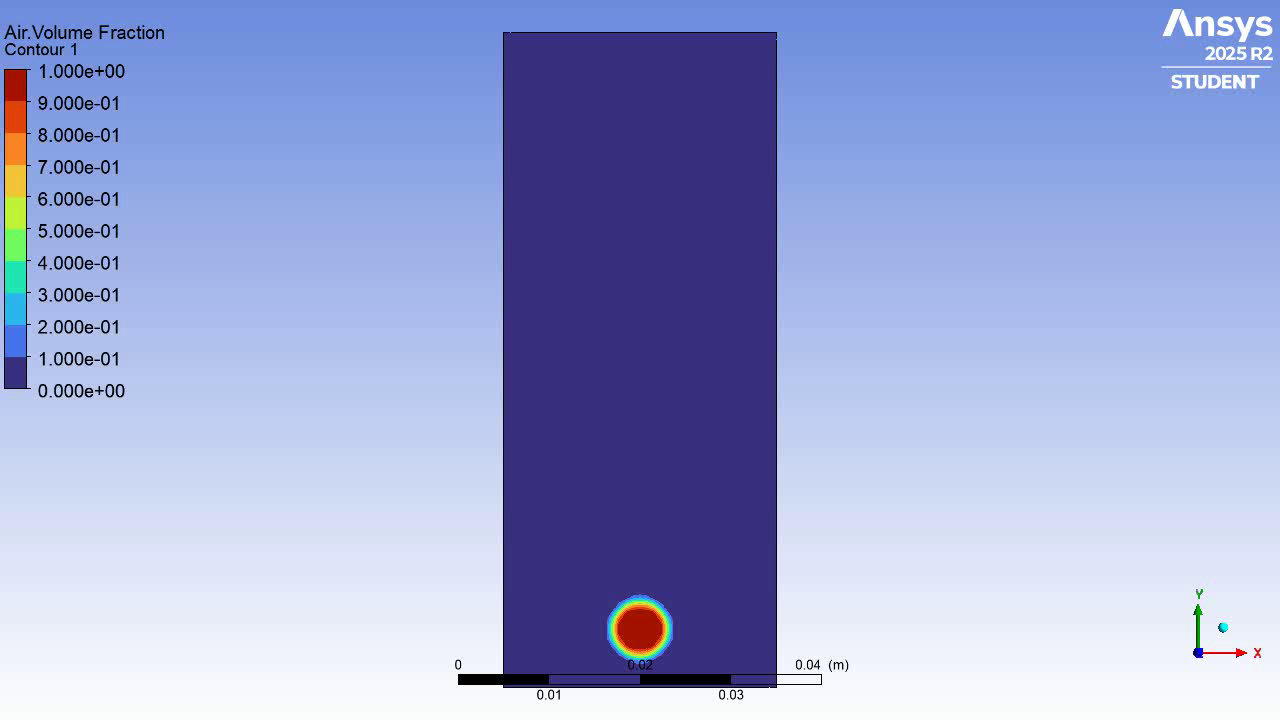
\includegraphics[width=0.24\linewidth]{../tut6_bubble_t1.png}
    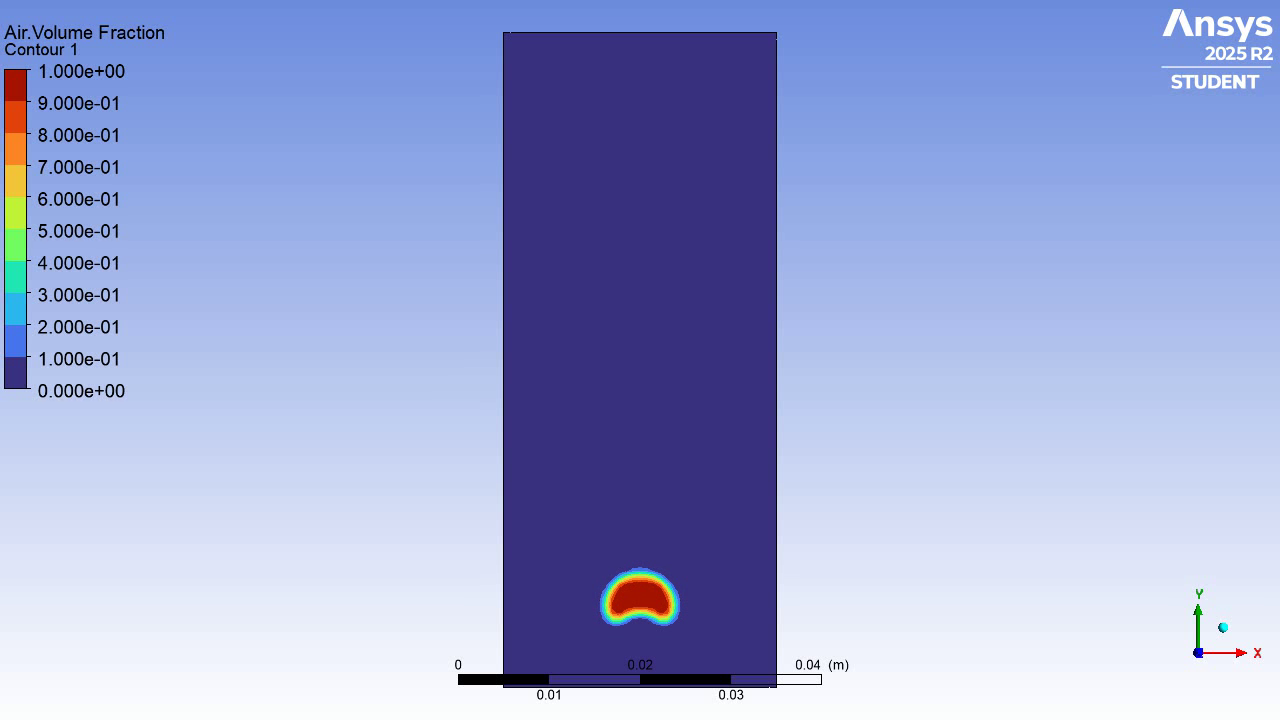
\includegraphics[width=0.24\linewidth]{../tut6_bubble_t2.png}
    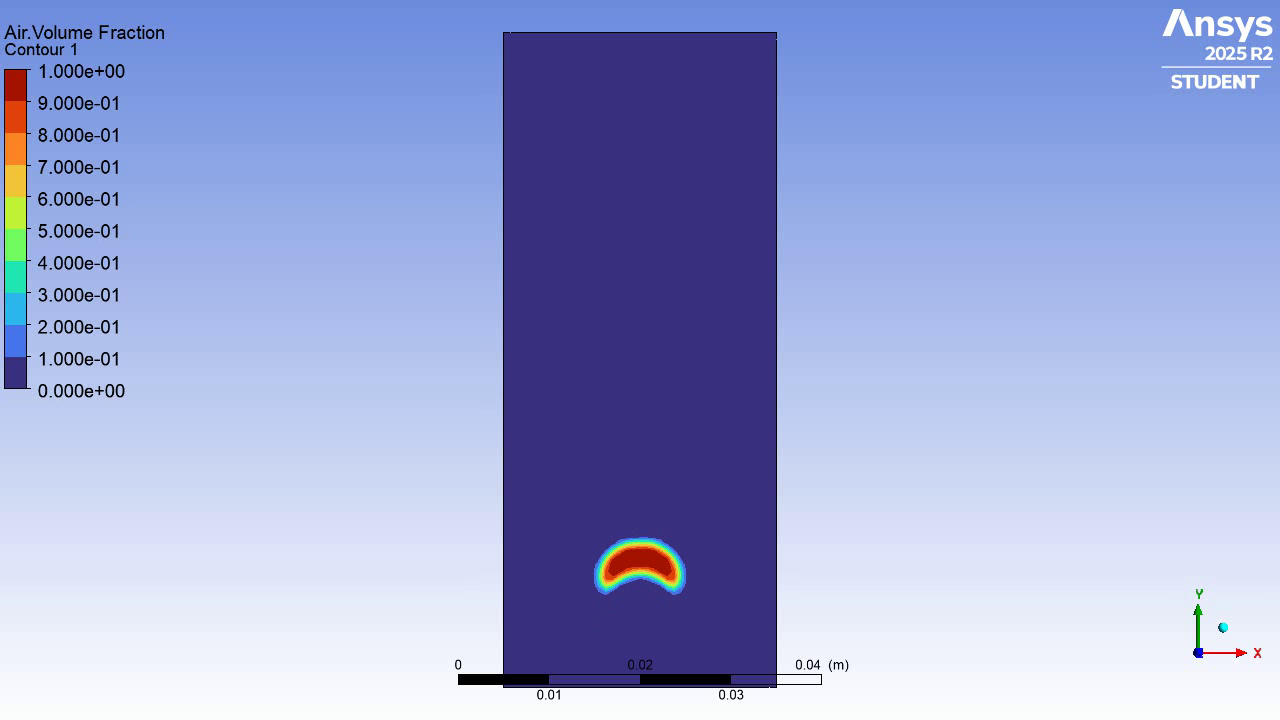
\includegraphics[width=0.24\linewidth]{../tut6_bubble_t3.png}
    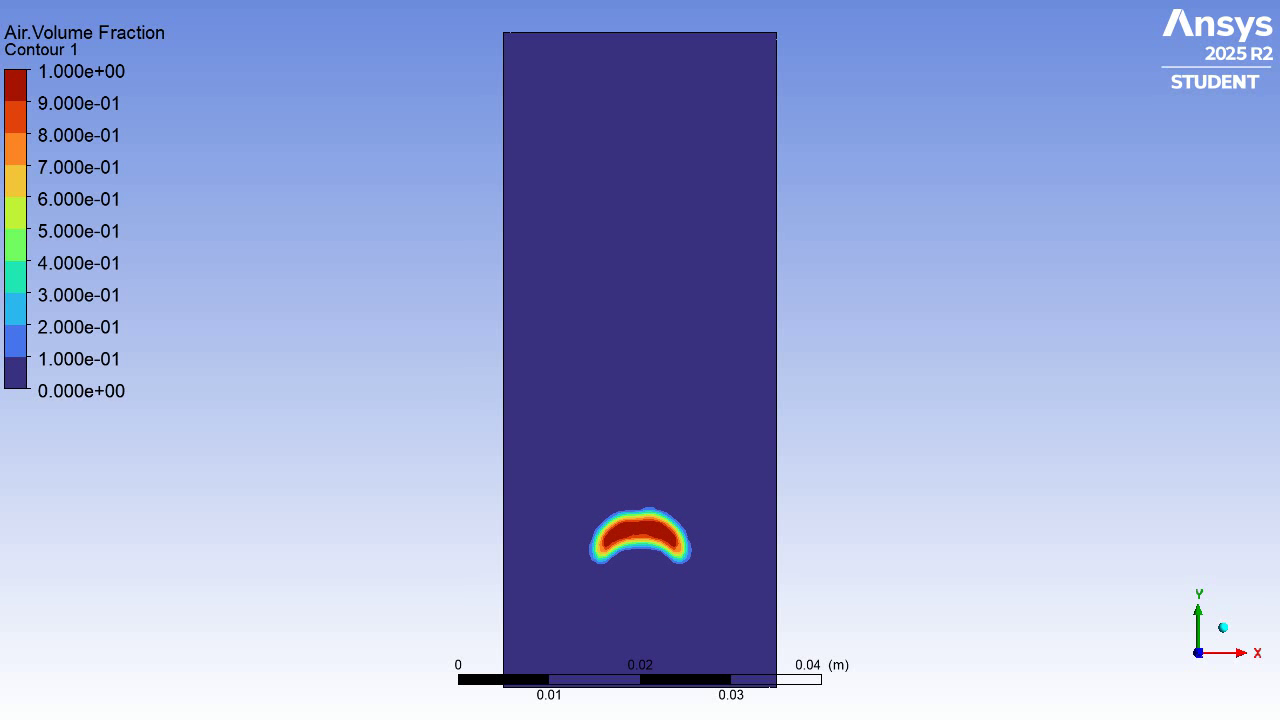
\includegraphics[width=0.24\linewidth]{../tut6_bubble_t4.png}
    \caption{Deformed bubble tracking over time using VOF.}
\end{figure}

\subsection{Analytical Validation}
Initially spherical, the bubble rapidly deforms into a dimpled/skirted shape as it accelerates. Hydrodynamic forces (buoyancy vs drag) quickly overcome the surface tension forces holding it spherical. For a $6$ mm bubble in water, the Morton number is calculated as $Mo \approx 5 \times 10^{-11}$ and the E\"{o}tv\"{o}s number is $Eo \approx 4.89$. According to the Clift et al. (1978) bubble shape diagram, these non-dimensional parameters place the bubble exactly in the "wobbling/ellipsoidal" regime, matching the simulated deformation perfectly.

The vertical velocity rises sharply and eventually asymptotes as drag balances buoyancy, achieving the terminal rise velocity. Analytically, using wave-speed approximations for this regime, the theoretical terminal velocity is estimated at $U_T \approx 0.23$ m/s, which aligns closely with the asymptote observed in the simulation results.

\subsection{Animation}
\textbf{Watch Animation:} \href{https://github.com/sajeev505/cll769_tuts_submission/blob/main/Tut_6/video.avi}{Click here to view the bubble rise video on GitHub!}

\end{document}
